% Options for packages loaded elsewhere
\PassOptionsToPackage{unicode}{hyperref}
\PassOptionsToPackage{hyphens}{url}
\PassOptionsToPackage{dvipsnames,svgnames,x11names}{xcolor}
%
\documentclass[
  letterpaper,
  11pt,
  english,
  singlespacing,
  headsepline]{MastersDoctoralThesis}

\usepackage{amsmath,amssymb}
\usepackage{iftex}
\ifPDFTeX
  \usepackage[T1]{fontenc}
  \usepackage[utf8]{inputenc}
  \usepackage{textcomp} % provide euro and other symbols
\else % if luatex or xetex
  \usepackage{unicode-math}
  \defaultfontfeatures{Scale=MatchLowercase}
  \defaultfontfeatures[\rmfamily]{Ligatures=TeX,Scale=1}
\fi
\usepackage{lmodern}
\ifPDFTeX\else  
    % xetex/luatex font selection
\fi
% Use upquote if available, for straight quotes in verbatim environments
\IfFileExists{upquote.sty}{\usepackage{upquote}}{}
\IfFileExists{microtype.sty}{% use microtype if available
  \usepackage[]{microtype}
  \UseMicrotypeSet[protrusion]{basicmath} % disable protrusion for tt fonts
}{}
\makeatletter
\@ifundefined{KOMAClassName}{% if non-KOMA class
  \IfFileExists{parskip.sty}{%
    \usepackage{parskip}
  }{% else
    \setlength{\parindent}{0pt}
    \setlength{\parskip}{6pt plus 2pt minus 1pt}}
}{% if KOMA class
  \KOMAoptions{parskip=half}}
\makeatother
\usepackage{xcolor}
\usepackage[paper=a4paper,inner=2.5cm,outer=3.8cm,bindingoffset=.5cm,top=1.5cm,bottom=1.5cm]{geometry}
\setlength{\emergencystretch}{3em} % prevent overfull lines
\setcounter{secnumdepth}{5}
% Make \paragraph and \subparagraph free-standing
\makeatletter
\ifx\paragraph\undefined\else
  \let\oldparagraph\paragraph
  \renewcommand{\paragraph}{
    \@ifstar
      \xxxParagraphStar
      \xxxParagraphNoStar
  }
  \newcommand{\xxxParagraphStar}[1]{\oldparagraph*{#1}\mbox{}}
  \newcommand{\xxxParagraphNoStar}[1]{\oldparagraph{#1}\mbox{}}
\fi
\ifx\subparagraph\undefined\else
  \let\oldsubparagraph\subparagraph
  \renewcommand{\subparagraph}{
    \@ifstar
      \xxxSubParagraphStar
      \xxxSubParagraphNoStar
  }
  \newcommand{\xxxSubParagraphStar}[1]{\oldsubparagraph*{#1}\mbox{}}
  \newcommand{\xxxSubParagraphNoStar}[1]{\oldsubparagraph{#1}\mbox{}}
\fi
\makeatother


\providecommand{\tightlist}{%
  \setlength{\itemsep}{0pt}\setlength{\parskip}{0pt}}\usepackage{longtable,booktabs,array}
\usepackage{calc} % for calculating minipage widths
% Correct order of tables after \paragraph or \subparagraph
\usepackage{etoolbox}
\makeatletter
\patchcmd\longtable{\par}{\if@noskipsec\mbox{}\fi\par}{}{}
\makeatother
% Allow footnotes in longtable head/foot
\IfFileExists{footnotehyper.sty}{\usepackage{footnotehyper}}{\usepackage{footnote}}
\makesavenoteenv{longtable}
\usepackage{graphicx}
\makeatletter
\newsavebox\pandoc@box
\newcommand*\pandocbounded[1]{% scales image to fit in text height/width
  \sbox\pandoc@box{#1}%
  \Gscale@div\@tempa{\textheight}{\dimexpr\ht\pandoc@box+\dp\pandoc@box\relax}%
  \Gscale@div\@tempb{\linewidth}{\wd\pandoc@box}%
  \ifdim\@tempb\p@<\@tempa\p@\let\@tempa\@tempb\fi% select the smaller of both
  \ifdim\@tempa\p@<\p@\scalebox{\@tempa}{\usebox\pandoc@box}%
  \else\usebox{\pandoc@box}%
  \fi%
}
% Set default figure placement to htbp
\def\fps@figure{htbp}
\makeatother

\usepackage[utf8]{inputenc} % Required for inputting international characters
%\usepackage[T1]{fontenc} % Output font encoding for international characters; causes problems for xelatex

%\usepackage{mathpazo} % Use the Palatino font by default

\usepackage[backend=bibtex, style=authoryear, natbib=true]{biblatex} % Use the bibtex backend with the authoryear citation style (which resembles APA)

\usepackage[autostyle=true]{csquotes} % Required to generate language-dependent quotes in the bibliography

\usepackage{setspace}

\usepackage{tikz}
\usetikzlibrary{calc}
\usetikzlibrary{calc,decorations.pathmorphing}
\usepackage{tocloft}
\usepackage{lscape} % For landscape pages
\usepackage{geometry} % For custom page layout
\usepackage{graphicx} % For including images
\usepackage{caption} % For custom captions
\usepackage{truncate}
\usepackage{lipsum} % For dummy text
\usepackage{xcolor} % To define and use colors
\usepackage{eso-pic} % For background images % For including images
\definecolor{textgray}{HTML}{595959}
\definecolor{greenTriangle}{HTML}{1f7549}
\definecolor{greenText}{HTML}{2DA86A}
\usepackage{tikz} % Load the TikZ package
\usepackage{tabularx}
\usepackage{fontspec} % To use system fonts like Arial
\PassOptionsToPackage{scaled}{helvet}
\usepackage{helvet}
\usetikzlibrary{patterns,patterns.meta} % LaTeX and plain TeX when using TikZ
\usepackage{titlesec}
\titleformat{\paragraph}[runin]{\normalfont\normalsize\bfseries}{\theparagraph}{1em}{}
\usepackage{multicol}
\usepackage{changepage}
%----------------------------------------------------------------------------------------
%	MARGINS
%----------------------------------------------------------------------------------------

\geometry{
	headheight=4ex,
	includehead,
	includefoot
}

\raggedbottom

\AtBeginDocument{
\hypersetup{pdftitle=\ttitle} % Set the PDF's title to your title
\hypersetup{pdfauthor=\authorname} % Set the PDF's author to your name
\hypersetup{pdfkeywords=\keywordnames} % Set the PDF's keywords to your keywords
}

\usepackage{tcolorbox}
\tcbset{
  colback=gray!10, % Background color (10% grey)
  colframe=gray!50, % Border color (50% grey)
  boxrule=0.5mm, % Border thickness
  arc=4mm, % Border radius
  left=1mm, % Left padding
  right=1mm, % Right padding
  top=1mm, % Top padding
  bottom=1mm, % Bottom padding
}

\renewcommand{\floatpagefraction}{0.8} % Allow floats to occupy up to 80% of a page
\renewcommand{\textfraction}{0.1}     % Allow text to occupy as little as 10% of a page
\renewcommand{\topfraction}{0.9}      % Allow up to 90% of the top of a page for floats
\renewcommand{\bottomfraction}{0.9}   % Allow up to 90% of the bottom of a page for floats

\newcommand{\startonrightwithgap}{%
  \clearpage
  % Check whether the current page is odd
  \ifodd\value{page}
    % -- We are on odd page X, so skip two pages (X+1, X+2):
    \thispagestyle{empty}\mbox{}\clearpage
    \thispagestyle{empty}\mbox{}\clearpage
  \else
    % -- We are on even page Y, so skip one page (Y+1):
    \thispagestyle{empty}\mbox{}\clearpage
  \fi
}

\newcommand{\startonleftwithgap}{%
  \clearpage
  \ifodd\value{page}
    % If the current page is odd, skip 3 blank pages
    \thispagestyle{empty}\mbox{}\clearpage
    \thispagestyle{empty}\mbox{}\clearpage
    \thispagestyle{empty}\mbox{}\clearpage
  \else
    % If the current page is even, skip 2 blank pages
    \thispagestyle{empty}\mbox{}\clearpage
    \thispagestyle{empty}\mbox{}\clearpage
  \fi
}
% 
% \newcommand{\startonrightwithgap}{%
%   \clearpage % End the current section cleanly
%   \ifodd\value{page} % Check if the current page is odd
%     \null\newpage % Add a blank page if odd
%     \thispagestyle{empty} % Ensure the blank page has no headers/footers
%   \else
%     \null\newpage % Add a blank page if even (this ensures X+1 is blank)
%     \thispagestyle{empty} % Ensure the blank page has no headers/footers
%     \null\newpage % Add another blank page for X+2
%     \thispagestyle{empty} % Ensure this blank page has no headers/footers
%   \fi
%   \cleardoublepage % Ensure the next section starts on a right (odd) page
% }

\newcommand{\chaptertopimage}{Chapter1/img/seagrasses.png}
\newcommand{\chapterbottomimage}{Chapter1/img/seagrasses.png}

\newcommand{\chaptertransition}{
    \clearpage
    \thispagestyle{empty}
    \null
    \newpage
}

\usepackage{geometry}  % presumably already in your preamble
% ... your usual margin setup, e.g.:
% \geometry{margin=1in}

\newcommand{\chaptertitlepage}[4]{%
  \chaptertransition
  \thispagestyle{empty}

  % Temporarily remove margins:
  \newgeometry{margin=0pt}

  \begin{center}
    % Top image, spanning full page width
    \includegraphics[width=\paperwidth]{#1}

    \vfill

    % Chapter number and title:
    {\Huge \textbf{Chapter #2: \\#3}}

    \vfill

    % Bottom image, also spanning full page width
    \includegraphics[width=\paperwidth]{#4}
  \end{center}

  % Restore your normal geometry:
  \restoregeometry
}

\makeatletter
\@ifpackageloaded{bookmark}{}{\usepackage{bookmark}}
\makeatother
\makeatletter
\@ifpackageloaded{caption}{}{\usepackage{caption}}
\AtBeginDocument{%
\ifdefined\contentsname
  \renewcommand*\contentsname{Table of contents}
\else
  \newcommand\contentsname{Table of contents}
\fi
\ifdefined\listfigurename
  \renewcommand*\listfigurename{List of Figures}
\else
  \newcommand\listfigurename{List of Figures}
\fi
\ifdefined\listtablename
  \renewcommand*\listtablename{List of Tables}
\else
  \newcommand\listtablename{List of Tables}
\fi
\ifdefined\figurename
  \renewcommand*\figurename{Figure}
\else
  \newcommand\figurename{Figure}
\fi
\ifdefined\tablename
  \renewcommand*\tablename{Table}
\else
  \newcommand\tablename{Table}
\fi
}
\@ifpackageloaded{float}{}{\usepackage{float}}
\floatstyle{ruled}
\@ifundefined{c@chapter}{\newfloat{codelisting}{h}{lop}}{\newfloat{codelisting}{h}{lop}[chapter]}
\floatname{codelisting}{Listing}
\newcommand*\listoflistings{\listof{codelisting}{List of Listings}}
\makeatother
\makeatletter
\makeatother
\makeatletter
\@ifpackageloaded{caption}{}{\usepackage{caption}}
\@ifpackageloaded{subcaption}{}{\usepackage{subcaption}}
\makeatother

\usepackage{bookmark}

\IfFileExists{xurl.sty}{\usepackage{xurl}}{} % add URL line breaks if available
\urlstyle{same} % disable monospaced font for URLs
\hypersetup{
  pdftitle={Caractérisation par télédétection multi-échelle de la végétation intertidale des côtes européennes en réponses aux pressions naturelles et anthropiques},
  pdfauthor={Simon Oiry},
  colorlinks=true,
  linkcolor={black},
  filecolor={Maroon},
  citecolor={black},
  urlcolor={black},
  pdfcreator={LaTeX via pandoc}}


\thesistitle{Caractérisation par télédétection multi-échelle de la
végétation intertidale des côtes européennes en réponses aux pressions
naturelles et
anthropiques} % Your thesis title, this is used in the title and abstract, print it elsewhere with \ttitle

% Modified section for multiple supervisors
\supervisor{Prof.~Laurent Barillé, Dr.~Pierre
Gernez} % Your supervisors' names, this will print all listed supervisors

\examiner{} % Your examiner's name, this is not currently used anywhere in the template, print it elsewhere with \examname
\degree{Doctor of Philosophy in Marine
Ecology} % Your degree name, this is used in the title page and abstract, print it elsewhere with \degreename
\author{Simon
Oiry} % Your name, this is used in the title page and abstract, print it elsewhere with \authorname
\addresses{} % Your address, this is not currently used anywhere in the template, print it elsewhere with \addressname

\subject{} % Your subject area, this is not currently used anywhere in the template, print it elsewhere with \subjectname
\keywords{} % Keywords for your thesis, this is not currently used anywhere in the template, print it elsewhere with \keywordnames
\university{University of
Nantes} % Your university's name, this is used in the title page and abstract, print it elsewhere with \univname
\department{Institut Des Substances et Organismes de la
Mer} % Your department's name, this is used in the title page and abstract, print it elsewhere with \deptname
\group{Remote Sensing, Benthic Ecology and Ecotoxicology
team} % Your research group's name and URL, this is used in the title page, print it elsewhere with \groupname
\faculty{Sciences \&
Techniques} % Your faculty's name and URL, this is used in the title page and abstract, print it elsewhere with \facname

\setcounter{tocdepth}{3} % The depth to which the document sections are printed to the table of contents
\begin{document}
%----------------------------------------------------------------------------------------
% FRONT MATTER CONFIGURATION
% Using roman page numbering style (i, ii, iii, iv...) for the pre-content pages
%----------------------------------------------------------------------------------------
\frontmatter

% Default to the plain heading style until the thesis style is called for the body content
\pagestyle{plain}

%----------------------------------------------------------------------------------------
% TITLE PAGE
%----------------------------------------------------------------------------------------
\newgeometry{top=0.5in, bottom=0.5in, left=0.5in, right=0.5in}

\begin{titlepage}

% Use Helvetica (Arial substitute)
\renewcommand{\familydefault}{\sfdefault}


\newcommand\BackgroundImage{%
    \put(0,3.5cm){%
        \parbox[b][\paperheight]{\paperwidth}{%
            \vfill
            
\includegraphics[width=\paperwidth]{Backgound_First_Page.png} % Replace with your image
            \vfill
        }%
    }%
}

% Use Arial font for the title page
\setsansfont{Arial}

\begin{tabularx}{\textwidth}{X X} % Two equally spaced columns
  \centering
\includegraphics[height=2cm]{LogoED.png} & 
  \centering
\includegraphics[height=2cm]{LogoUN.jpg} \\
\end{tabularx}

% Add the background image
\AddToShipoutPictureBG*{%
    \BackgroundImage
}

\vspace{1.2cm}

% Custom font sizes for "THESE DE DOCTORAT"
{\LARGE {\Huge T}HESE DE DOCTORAT}

\vspace{1.8cm}
% Custom font sizes for "NANTES UNIVERSITE"
{\fontsize{14}{18}\selectfont NANTES UNIVERSITE} \\

{\large E}COLE {\large D}OCTORALE N° 642


{\fontsize{12}{16}\selectfont \textit{Ecole doctorale Végétal, Animal, Aliment, Mer, Environnement}}

{\fontsize{12}{16}\selectfont Spécialité : Biologie et écologie marine} \\\\\\

{\fontsize{12}{16}\ Par}
\vspace{0.2cm}

\hspace{0.7cm}{\fontsize{20}{24}\selectfont \textbf{Simon OIRY}} \\

\parbox{17cm}{
{\fontsize{16}{20}\selectfont \textbf{Caractérisation par télédétection multi-échelle de la végétation intertidale des côtes européennes en réponses aux pressions naturelles et anthropiques} }
}\\\\

{\fontsize{11}{15}\selectfont \textbf{Thèse présentée et soutenue à Nantes, le 15 mai 2025}}

{\fontsize{11}{15}\selectfont \textbf{Unité de Recherche: Institut Des Substances et Organismes de la Mer}}
\\\\\\

{\fontsize{12}{16}\selectfont \textbf{Rapporteurs avant soutenance :}}

\begin{tabular}{@{}l l l@{}}
    {\fontsize{10}{14}\selectfont \textcolor{textgray}{Antoine Collin}} & 
    {\fontsize{10}{14}\selectfont \textcolor{textgray}{Maitre de conférences}} & 
    {\fontsize{10}{14}\selectfont \textcolor{textgray}{Ecole Pratique des Hautes Etudes, Dinard}} \\

    {\fontsize{10}{14}\selectfont \textcolor{textgray}{Rodney Foster}} & 
    {\fontsize{10}{14}\selectfont \textcolor{textgray}{Professeur}} & 
    {\fontsize{10}{14}\selectfont \textcolor{textgray}{Université de Hull, Royaume-Uni}} \\
\end{tabular}\\\\

{\fontsize{12}{16}\selectfont \textbf{Composition du Jury : }}

\begin{tabular}{@{}l l l l@{}}
    {\fontsize{10}{14}\selectfont \textcolor{textgray}{Président :}} & 
    {\fontsize{10}{14}\selectfont \textcolor{textgray}{ }} & 
    {\fontsize{10}{14}\selectfont \textcolor{textgray}{ }} & 
    {\fontsize{10}{14}\selectfont \textcolor{textgray}{ }} \\

    {\fontsize{10}{14}\selectfont \textcolor{textgray}{Examinateurs :}} & 
    {\fontsize{10}{14}\selectfont \textcolor{textgray}{Antoine Collin}} & 
    {\fontsize{10}{14}\selectfont \textcolor{textgray}{Maitre de conférences}} & 
    {\fontsize{10}{14}\selectfont \textcolor{textgray}{Ecole Pratique des Hautes Etudes, Dinard}} \\
    
    {\fontsize{10}{14}\selectfont \textcolor{textgray}{}} & 
    {\fontsize{10}{14}\selectfont \textcolor{textgray}{Rodney Foster}} & 
    {\fontsize{10}{14}\selectfont \textcolor{textgray}{Professeur}} & 
    {\fontsize{10}{14}\selectfont \textcolor{textgray}{Université de Hull, Royaume-Uni}} \\

    {\fontsize{10}{14}\selectfont \textcolor{textgray}{}} & 
    {\fontsize{10}{14}\selectfont \textcolor{textgray}{Evangelos Spyrakos}} & 
    {\fontsize{10}{14}\selectfont \textcolor{textgray}{Professeur}} & 
    {\fontsize{10}{14}\selectfont \textcolor{textgray}{Université de Stirling, Royaume-Uni}} \\

    {\fontsize{10}{14}\selectfont \textcolor{textgray}{}} & 
    {\fontsize{10}{14}\selectfont \textcolor{textgray}{Barbara Ondiviela}} & 
    {\fontsize{10}{14}\selectfont \textcolor{textgray}{Senior scientist}} & 
    {\fontsize{10}{14}\selectfont \textcolor{textgray}{Université de Cantabrie, Espagne}} \\

    {\fontsize{10}{14}\selectfont \textcolor{textgray}{Dir. de thèse :}} & 
    {\fontsize{10}{14}\selectfont \textcolor{textgray}{Laurent Barillé}} & 
    {\fontsize{10}{14}\selectfont \textcolor{textgray}{Professeur}} & 
    {\fontsize{10}{14}\selectfont \textcolor{textgray}{Nantes Université}} \\

    {\fontsize{10}{14}\selectfont \textcolor{textgray}{Co-dir. de thèse :}} & 
    {\fontsize{10}{14}\selectfont \textcolor{textgray}{Pierre Gernez}} & 
    {\fontsize{10}{14}\selectfont \textcolor{textgray}{Maitre de conférence}} & 
    {\fontsize{10}{14}\selectfont \textcolor{textgray}{Nantes Université}} \\
\end{tabular} \\\\

{\fontsize{11}{15}\selectfont \textbf{Invitée : }}


\begin{tabular}{@{}l l l@{}}
    {\fontsize{10}{14}\selectfont \textcolor{textgray}{Federica Braga}} & 
    {\fontsize{10}{14}\selectfont \textcolor{textgray}{Senior Researcher}} & 
    {\fontsize{10}{14}\selectfont \textcolor{textgray}{Conseil Supérieur de la Recherche, Venise, Italie}} \\

\end{tabular}
\end{titlepage}

% Restore the default margins for the rest of the document
\restoregeometry

% Reset to serif font for the rest of the document
\renewcommand{\familydefault}{\rmdefault}


%----------------------------------------------------------------------------------------
% DECLARATION PAGE
%----------------------------------------------------------------------------------------

%----------------------------------------------------------------------------------------
% QUOTATION PAGE (IF ANY)
%----------------------------------------------------------------------------------------

%----------------------------------------------------------------------------------------
% ABSTRACT PAGE
%----------------------------------------------------------------------------------------
% %   \clearpage
%   \begin{abstract}
%     \addchaptertocentry{\abstractname}  % Add the abstract to the table of contents
%     To Be Written
%   \end{abstract}
% 
%----------------------------------------------------------------------------------------
% ACKNOWLEDGEMENTS
%----------------------------------------------------------------------------------------
  \startonrightwithgap
  \begin{acknowledgements}
    \addchaptertocentry{\acknowledgementname} % Add the acknowledgements to the table of contents
          

Ce parcours de doctorat a été long, difficile et parfois épuisant, mais il a également été rempli de moments enrichissants et de personnes incroyables qui ont rendu tout cela digne d'intérêt.

Tout d'abord, je tiens à exprimer ma plus profonde gratitude à mon directeur de thèse, Laurent Barillé. Merci pour tes conseils, ta patience et ton soutien sans faille tout au long de ce processus. Merci pour toute la liberté que tu m'as accordée pendant ces années. Ton expertise et tes encouragements m'ont poussé à m'améliorer à chaque étape, même lorsque j'avais des doutes. J'ai appris énormément sous ta direction, et je suis vraiment reconnaissant de la confiance que tu m'as accordée. Un merci particulier pour ton aide avec toutes les démarches administratives — je sais que j'ai été paresseux à ce sujet, et j'apprécie sincèrement ta patience !

Un grand merci également à mon co-directeur, Pierre Gernez, pour tes conseils avisés, tes retours constructifs et ton soutien constant. Ta perspective m'a toujours aidé à prendre du recul et à voir les choses plus clairement, et j'ai profondément apprécié nos discussions.

J'ai eu une chance incroyable de travailler aux côtés de Bede Davies, dont la générosité en termes de temps et de connaissances a dépassé tout ce que j'aurais pu espérer d'un collègue. Bede, collaborer avec toi a été l'un des meilleurs aspects de ce doctorat — ta patience et ton dévouement ont rendu même les défis de recherche les plus difficiles plus faciles à gérer.

Je tiens également à remercier sincèrement Philippe Rosa, qui a été un véritable sauveur pendant les travaux de terrain. Philippe, tu étais toujours là, prêt à aider, résoudre des problèmes ou simplement partager un éclat de rire quand les choses allaient inévitablement de travers sur le terrain.

Sur un plan plus personnel, je dois une immense gratitude à Laura Zoffoli. Merci d'avoir supporté les nuits tardives, le stress et les conversations interminables sur les herbiers et la télédétection. Ton soutien et ta patience ont été essentiels pour moi, et je n'aurais pas pu accomplir cela sans toi.

Enfin, à ma famille — merci de m'avoir toujours cru, même lorsque je ne croyais pas en moi. Vos encouragements, votre amour et vos rappels qu'il y a une vie en dehors de la recherche ont été une source constante de force. Je suis tellement chanceux de vous avoir à mes côtés.

À tous ceux qui ont fait partie de ce parcours d'une manière ou d'une autre — merci.


      \end{acknowledgements}

%----------------------------------------------------------------------------------------
% LIST OF CONTENTS/FIGURES/TABLES
%----------------------------------------------------------------------------------------
\setlength{\cftsecindent}{0.5em}        % Less indentation for sections
\setlength{\cftsubsecindent}{1em}       % Less indentation for subsections
\setlength{\cftsubsubsecindent}{1.5em}  % Less indentation for subsubsections
\renewcommand{\cftfigpresnum}{Figure~}
\renewcommand{\cfttabpresnum}{Table~}
\renewcommand{\cftfigaftersnum}{:~}  % Add ": " after the figure number
\renewcommand{\cfttabaftersnum}{:~}  % Add ": " after the table number  % Prefix for tables
\setlength{\cftbeforefigskip}{0.5em}  % Space between figure entries
\setlength{\cftbeforetabskip}{0.5em} % Space between table entries
\setlength{\cftfignumwidth}{5em} % Adjust width for figure numbers
\setlength{\cfttabnumwidth}{5em} % Adjust width for table numbers
\setlength{\cftfigindent}{0em}    % Indentation for figure captions
\setlength{\cfttabindent}{0em}    % Indentation for table captions
\startonrightwithgap
\begingroup
\hypersetup{linkcolor=black}
\startonrightwithgap
\tableofcontents  
\startonrightwithgap
\listoffigures
\startonrightwithgap
\listoftables 
\endgroup

%----------------------------------------------------------------------------------------
% ABBREVIATIONS (IF ANY)
%----------------------------------------------------------------------------------------
  % \addchaptertocentry{\abbreviationsname}
  % \label{abbreviations}
  \startonrightwithgap
  \begin{abbreviations}{p{0.2\textwidth} p{0.75\textwidth}} % Adjust the widths as needed
  ASI & \textbf{A}genzia \textbf{S}paziale \textbf{I}taliana \\
  ANOSIM & \textbf{A}nalysis of \textbf{S}imilarity \\
  AHW & \textbf{A}tmospheric \textbf{H}eat\textbf{w}ave \\
  BOA & \textbf{B}ottom of \textbf{A}tmosphere \\
  BPI & \textbf{B}rown \textbf{P}igment \textbf{I}ndex \\
  Chla & \textbf{Chl}orophyll-\textbf{a} \\
  Chlb & \textbf{Chl}orophyll-\textbf{b} \\
  Chlc & \textbf{Chl}orophyll-\textbf{c} \\
  CMEMS & \textbf{C}opernicus \textbf{M}arine \textbf{E}nvironment \textbf{M}onitoring \textbf{S}ervice \\
  dGPS & \textbf{d}ifferential \textbf{G}PS \\
  DHM & \textbf{D}igital \textbf{H}eight \textbf{M}odel \\
  DSM & \textbf{D}igital \textbf{S}urface \textbf{M}odel \\
  DTM & \textbf{D}igital \textbf{T}errain \textbf{M}odel \\
  DPA & \textbf{D}iphenylamine \\
  DISCOV & \textbf{D}rone \textbf{I}ntertidal \textbf{S}ubstrate \textbf{C}lassification \textbf{O}f \textbf{V}egetation \\
  DLS2 & \textbf{D}ownwelling \textbf{L}ight \textbf{S}ensor \\
  EO & \textbf{E}arth \textbf{O}bservation \\
  EMR & \textbf{E}lectromagnetic \textbf{R}adiation \\
  EBVs & \textbf{E}ssential \textbf{B}iodiversity \textbf{V}ariables \\
  EOVs & \textbf{E}ssential \textbf{O}cean \textbf{V}ariables \\
  ESA & \textbf{E}uropean \textbf{S}pace \textbf{A}gency \\
  EU & \textbf{E}uropean \textbf{U}nion \\
  EPS & \textbf{E}xtracellular \textbf{P}olymeric \textbf{S}ubstances \\
  IGN & \textbf{I}nstitut \textbf{N}ational de l’information \textbf{G}eographique et forestiere \\
  FO & \textbf{F}ront \textbf{O}verlap \\
  FWHM & \textbf{F}ull \textbf{W}idth at \textbf{H}alf \textbf{M}aximum \\
  GAM & \textbf{G}eneralized \textbf{A}dditive \textbf{M}odel \\
  GLM & \textbf{G}eneralized \textbf{L}inear \textbf{M}odel \\
  GLMM & \textbf{G}eneralized \textbf{L}inear \textbf{M}ixed \textbf{M}odel \\
  GBIF & \textbf{G}lobal \textbf{B}iodiversity \textbf{I}nformation \textbf{F}acility \\
  GOOS & \textbf{G}lobal \textbf{O}cean \textbf{O}bserving \textbf{S}ystem \\
  GLI & \textbf{G}reen \textbf{L}eaf \textbf{I}ndex \\
  GVA & \textbf{G}ross \textbf{V}alue \textbf{A}dded \\
  HSPs & \textbf{H}eat-\textbf{S}hock \textbf{P}roteins \\
  HIDF & \textbf{H}eatwave \textbf{I}ntensity \textbf{D}uration \textbf{F}requency \\
  HPLC & \textbf{H}igh \textbf{P}erformance \textbf{L}iquid \textbf{C}hromatography \\
  HiRI & \textbf{H}igh-resolution \textbf{I}mager \\
  HW & \textbf{H}eat\textbf{W}ave \\
  HYC & \textbf{H}yperspectral \textbf{C}amera \\
  ICE CREAMS & \textbf{I}ntertidal \textbf{C}lassification of \textbf{E}urope: \textbf{C}ategorising \textbf{R}eflectance of \textbf{E}merged \textbf{A}reas of \textbf{M}arine vegetation with \textbf{S}entinel2 \\
  IR & \textbf{I}nfrared \\
  IFOV & \textbf{I}nstantaneous \textbf{F}ield of \textbf{V}iew \\
  IGN & \textbf{I}nstitut \textbf{N}ational de l’Information \textbf{G}éographique et \textbf{F}orestiere (2024a) \\
  IPBES & \textbf{I}ntergovernmental \textbf{S}cience-\textbf{P}olicy \textbf{P}latform on \textbf{B}iodiversity and \textbf{E}cosystem \textbf{S}ervices \\
  IAS & \textbf{I}nvasive \textbf{A}lien \textbf{S}pecies \\
  LiDAR & \textbf{L}ight \textbf{D}etection and \textbf{R}anging \\
  MSFD & \textbf{M}arine \textbf{S}trategy \textbf{F}ramework \textbf{D}irective \\
  ML & \textbf{M}achine \textbf{L}earning \\
  MHW & \textbf{M}arine \textbf{H}eat\textbf{w}ave \\
  PRISMA & \textbf{Pr}ecursore \textbf{I}per\textbf{s}pecttrale della \textbf{M}issione \textbf{A}pplicativa \\
  PAR & \textbf{P}hotosynthetically \textbf{A}ctive \textbf{R}adiation \\ 
  SST & \textbf{S}ea \textbf{S}urface \textbf{T}emperature
\end{abbreviations}


%----------------------------------------------------------------------------------------
% PHYSICAL CONSTANTS/OTHER DEFINITIONS (IF ANY)
%----------------------------------------------------------------------------------------

%----------------------------------------------------------------------------------------
% SYMBOLS (IF ANY)
%----------------------------------------------------------------------------------------
  % \addchaptertocentry{\symbolsname}
  \startonrightwithgap
  \begin{symbols}{ll} % Include a list of Symbols (a three column table)

  FN$_i$ & False negative relative to the class $i$ \\
  FP$_i$ & False positive relative to the class $i$ \\
  $h_{\text{sensor}}$ & Sensor dimension (height) in the flight direction \\
  TN$_i$ & True negatives relative to the class $i$ \\
  TP$_i$ & True positives relative to the class $i$ \\
  $L_{down}$ & Downwelling radiance \\
  $L_{up}$ & Upwelling radiance \\
  $R_{BOA}$ & Reflectance at the bottom of atmosphere \\
  $R_i(\lambda)$ & Reflectance of spectrum $i$ at a specific wavelength $\lambda$ \\
  $R^*_i(\lambda)$ & Standardised $R$ of spectrum $i$ at wavelength $\lambda$ \\
  $d_{fl}$ & Distance between two adjacent flight lines \\
  $w_{\text{sensor}}$ & Sensor dimension (width) perpendicular to the flight direction \\
  $L$ & Radiance \\
  max($R_i$) & Maximum reflectance value at spectrum $i$ \\
  min($R_i$) & Minimum reflectance value at spectrum $i$ \\
  $h$ & Flight altitude above the ground \\
  $R$ & Reflectance \\
  $R''(\lambda_i)$ & Second derivative at the wavelength i $\lambda_i$\\
  $f$ & Camera focal length \\
  $v_g$ & Ground speed of the drone \\
  $\Delta t$ & Time interval between consecutive photos \\
  $\Delta \lambda$ & Uniform spectral sampling interval \\
  $\lambda$ & Wavelength \\

\end{symbols}

%----------------------------------------------------------------------------------------
% DEDICATION (IF ANY)
%----------------------------------------------------------------------------------------

%----------------------------------------------------------------------------------------
% MAIN CONTENT
%----------------------------------------------------------------------------------------
\mainmatter % Begin numeric (1,2,3...) page numbering
% Return the page headers back to the "thesis" style
\pagestyle{thesis}
% Define some commands to keep the formatting separated from the content 
\newcommand{\keyword}[1]{\textbf{#1}}
\newcommand{\tabhead}[1]{\textbf{#1}}
\newcommand{\code}[1]{\texttt{#1}}
\newcommand{\file}[1]{\texttt{\bfseries#1}}
\newcommand{\option}[1]{\texttt{\itshape#1}}
% \renewcommand{\chaptermark}[1]{\markboth{#1}{}}


\bookmarksetup{startatroot}

\chapter*{Preface}\label{preface}
\addcontentsline{toc}{chapter}{Preface}

\markboth{Preface}{Preface}

This PhD work was carried out at Nantes University between 2022 and
2024, within the ``Remote Sensing, Benthic Ecology and Ecotoxicology''
(RSBE²) team of the Institute of Marine Substances and Organisms
(ISOMer). This thesis was funded by the Ministry of Research and Higher
Education and supervised by the doctoral school ``Plant, Animal, Food,
Sea, Environment'' (VAAME).

\section*{Scientific papers}\label{scientific-papers}
\addcontentsline{toc}{section}{Scientific papers}

\markright{Scientific papers}

\begin{itemize}
\item
  \textbf{Oiry, S}., Davies, B. F. R., Rosa, P., Debly, A., Zoffoli, M.
  L., Barillé, A.-L., Harin, N., Román, M., Gernez, P., \& Barillé, L.
  (Submitted). Heatwave impacts on intertidal seagrass reflectance: From
  laboratory experiment to satellite mapping of Seagrass Heat Shock
  Index.
\item
  \textbf{Oiry, S.}, Davies, B. F. R., Stiger-Pouvreau, V., Gernez, P.,
  \& Barillé, L. (Submitted). Mapping the distribution of the alien
  invasive \emph{Gracilaria vermiculophylla} at the site of its First
  European Observation.
\item
  Barillé, L., Paterson, I. L. R., \textbf{Oiry, S.}, Aris, A.,
  Cook-Cottier, E. J., \& Nurdin, N. (2025). Variability of
  \emph{Kappaphycus alvarezii} cultivation in South-Sulawesi (Indonesia)
  related to the monsoon shift: Water quality, growth and colour
  quantification. \emph{Aquaculture Reports}, 40, 102557.
  https://doi.org/10.1016/j.aqrep.2024.102557
\item
  \textbf{Oiry, S.}, Davies, B. F. R., Sousa, A. I., Rosa, P., Zoffoli,
  M. L., Brunier, G., Gernez, P., \& Barillé, L. (2024). Discriminating
  Seagrasses from Green Macroalgae in European Intertidal Areas Using
  High-Resolution Multispectral Drone Imagery.~\emph{Remote
  Sensing},~\emph{16}(23), 4383. https://doi.org/10.3390/rs16234383
\item
  Román, A., \textbf{Oiry, S.}, Davies, B. F. R., Rosa, P., Gernez, P.,
  Tovar-Sánchez, A., Navarro, G., Méléder, V., \& Barillé, L. (2024).
  Mapping intertidal microphytobenthic biomass with very high-resolution
  remote sensing imagery in an estuarine system. \emph{Science of The
  Total Environment}, 955, 177025.
  https://doi.org/10.1016/j.scitotenv.2024.177025
\item
  Davies, B. F. R., \textbf{Oiry, S.}, Rosa, P., Zoffoli, M. L., Sousa,
  A. I., Thomas, O. R., Smale, D. A., Austen, M. C., Biermann, L.,
  Attrill, M. J., Roman, A., Navarro, G., Barillé, A.-L., Harin, N.,
  Clewley, D., Martinez-Vicente, V., Gernez, P., \& Barillé, L. (2024).
  Intertidal seagrass extent from Sentinel-2 time-series show distinct
  trajectories in Western Europe. \emph{Remote Sensing of Environment},
  312, 114340. https://doi.org/10.1016/j.rse.2024.114340
\item
  Davies, B. F. R., \textbf{Oiry, S.}, Rosa, P., Zoffoli, M. L., Sousa,
  A. I., Thomas, O. R., Smale, D. A., Austen, M. C., Biermann, L.,
  Attrill, M. J., \& others. (2024). A sentinel watching over
  inter-tidal seagrass phenology across Western Europe and North Africa.
  \emph{Communications Earth \& Environment}, 5(1), 382.
  https://doi.org/10.1038/s43247-024-382
\item
  Nurdin, N., Alevizos, E., Syamsuddin, R., Asis, H., Zainuddin, E. N.,
  Aris, A., \textbf{Oiry, S.}, Brunier, G., Komatsu, T., \& Barillé, L.
  (2023). Precision Aquaculture Drone Mapping of the Spatial
  Distribution of~\emph{Kappaphycus alvarezii}~Biomass and
  Carrageenan.~\emph{Remote Sensing},~\emph{15}(14), 3674.
  https://doi.org/10.3390/rs15143674
\item
  Román, A., Prasyad, H.,\textbf{Oiry, S.}, Davies, B. F. R., Brunier,
  G., \& Barillé, L. (2023). Mapping intertidal oyster farms using
  unmanned aerial vehicles (UAV) high-resolution multispectral data.
  \emph{Estuarine, Coastal and Shelf Science}, 291, 108432.
  https://doi.org/10.1016/j.ecss.2023.108432
\item
  Davies, B. F. R., Gernez, P., Geraud, A., \textbf{Oiry, S.}, Rosa, P.,
  Zoffoli, M. L., \& Barillé, L. (2023). Multi- and hyperspectral
  classification of soft-bottom intertidal vegetation using a spectral
  library for coastal biodiversity remote sensing. \emph{Remote Sensing
  of Environment}, 290, 113554.
  https://doi.org/10.1016/j.rse.2023.113554
\item
  Zoffoli, M.L., Gernez, P., \textbf{Oiry, S.}, Godet, L., Dalloyau, S.,
  Davies, B.F.R. and Barillé, L. (2023), Remote sensing in seagrass
  ecology: coupled dynamics between migratory herbivorous birds and
  intertidal meadows observed by satellite during four decades.
  \emph{Remote Sens Ecol Conserv}, 9:
  420-433.~\url{https://doi.org/10.1002/rse2.319}
\item
  Brunier, G., \textbf{Oiry, S}., Lachaussée, N., Barillé, L., Le
  Fouest, V., \& Méléder, V. (2022). A Machine-Learning Approach to
  Intertidal Mudflat Mapping Combining Multispectral Reflectance and
  Geomorphology from UAV-Based Monitoring.~\emph{Remote
  Sensing},~\emph{14}(22), 5857. https://doi.org/10.3390/rs14225857
\item
  Brunier, G., \textbf{Oiry, S.}, Gruet, Y., Dubois, S. F., \& Barillé,
  L. (2022). Topographic Analysis of Intertidal Polychaete Reefs
  (Sabellaria alveolata) at a Very High Spatial Resolution. \emph{Remote
  Sensing}, 14(2), 307. https://doi.org/10.3390/rs14020307
\end{itemize}

\section*{Presentations to International
Conferences}\label{presentations-to-international-conferences}
\addcontentsline{toc}{section}{Presentations to International
Conferences}

\markright{Presentations to International Conferences}

\begin{itemize}
\item
  Effect of Marine and Atmospheric Heatwaves on Reflectance and Pigment
  Composition of Intertidal \emph{Zostera noltei} (February 2025);
  BioSpace25 - Biodiversity insight from Space, Frascati, Italy; Oral
  presentation
\item
  Discriminating Seagrasses From Green Macroalgae in European Intertidal
  Areas using High Resolution Multispectral Drone Imagery (17 - 21 June
  2024); Word Seagrass Conference, Napoli, Italy; Poster
\item
  Remote Sensing discrimination of seagrass and green macroalgae:
  hyperspectral library and drone-mounted multispectral camera (22 - 24
  November 2023); EC-ESA Joint Earth System Science Initiative,
  Frascati, Italy; Poster
\item
  Precision aquaculture drone mapping of the spatial distribution of
  \emph{Kappaphycus alvarezii} biomass and carrageenan (20 - 26 August
  2023); 8th European Phycological Congress, Brest, France ; Oral
  presentation
\item
  Remote Sensing discrimination of seagrass and green macroalgae:
  hyperspectral library and drone-mounted multispectral camera (20 - 26
  August 2023); 8th European Phycological Congress, Brest, France ;
  Poster
\item
  Topographic analysis of intertidal polychaete reefs (Sabellaria
  alveolata) using very high resolution UAV remote sensing (23 - 27 may
  2022); Living Planet Symposium, Bonn, Germany ; Poster
\end{itemize}

\section*{Project related to the
thesis.}\label{project-related-to-the-thesis.}
\addcontentsline{toc}{section}{Project related to the thesis.}

\markright{Project related to the thesis.}

\subsection*{BiCOME}\label{bicome}
\addcontentsline{toc}{subsection}{BiCOME}

\begin{center}
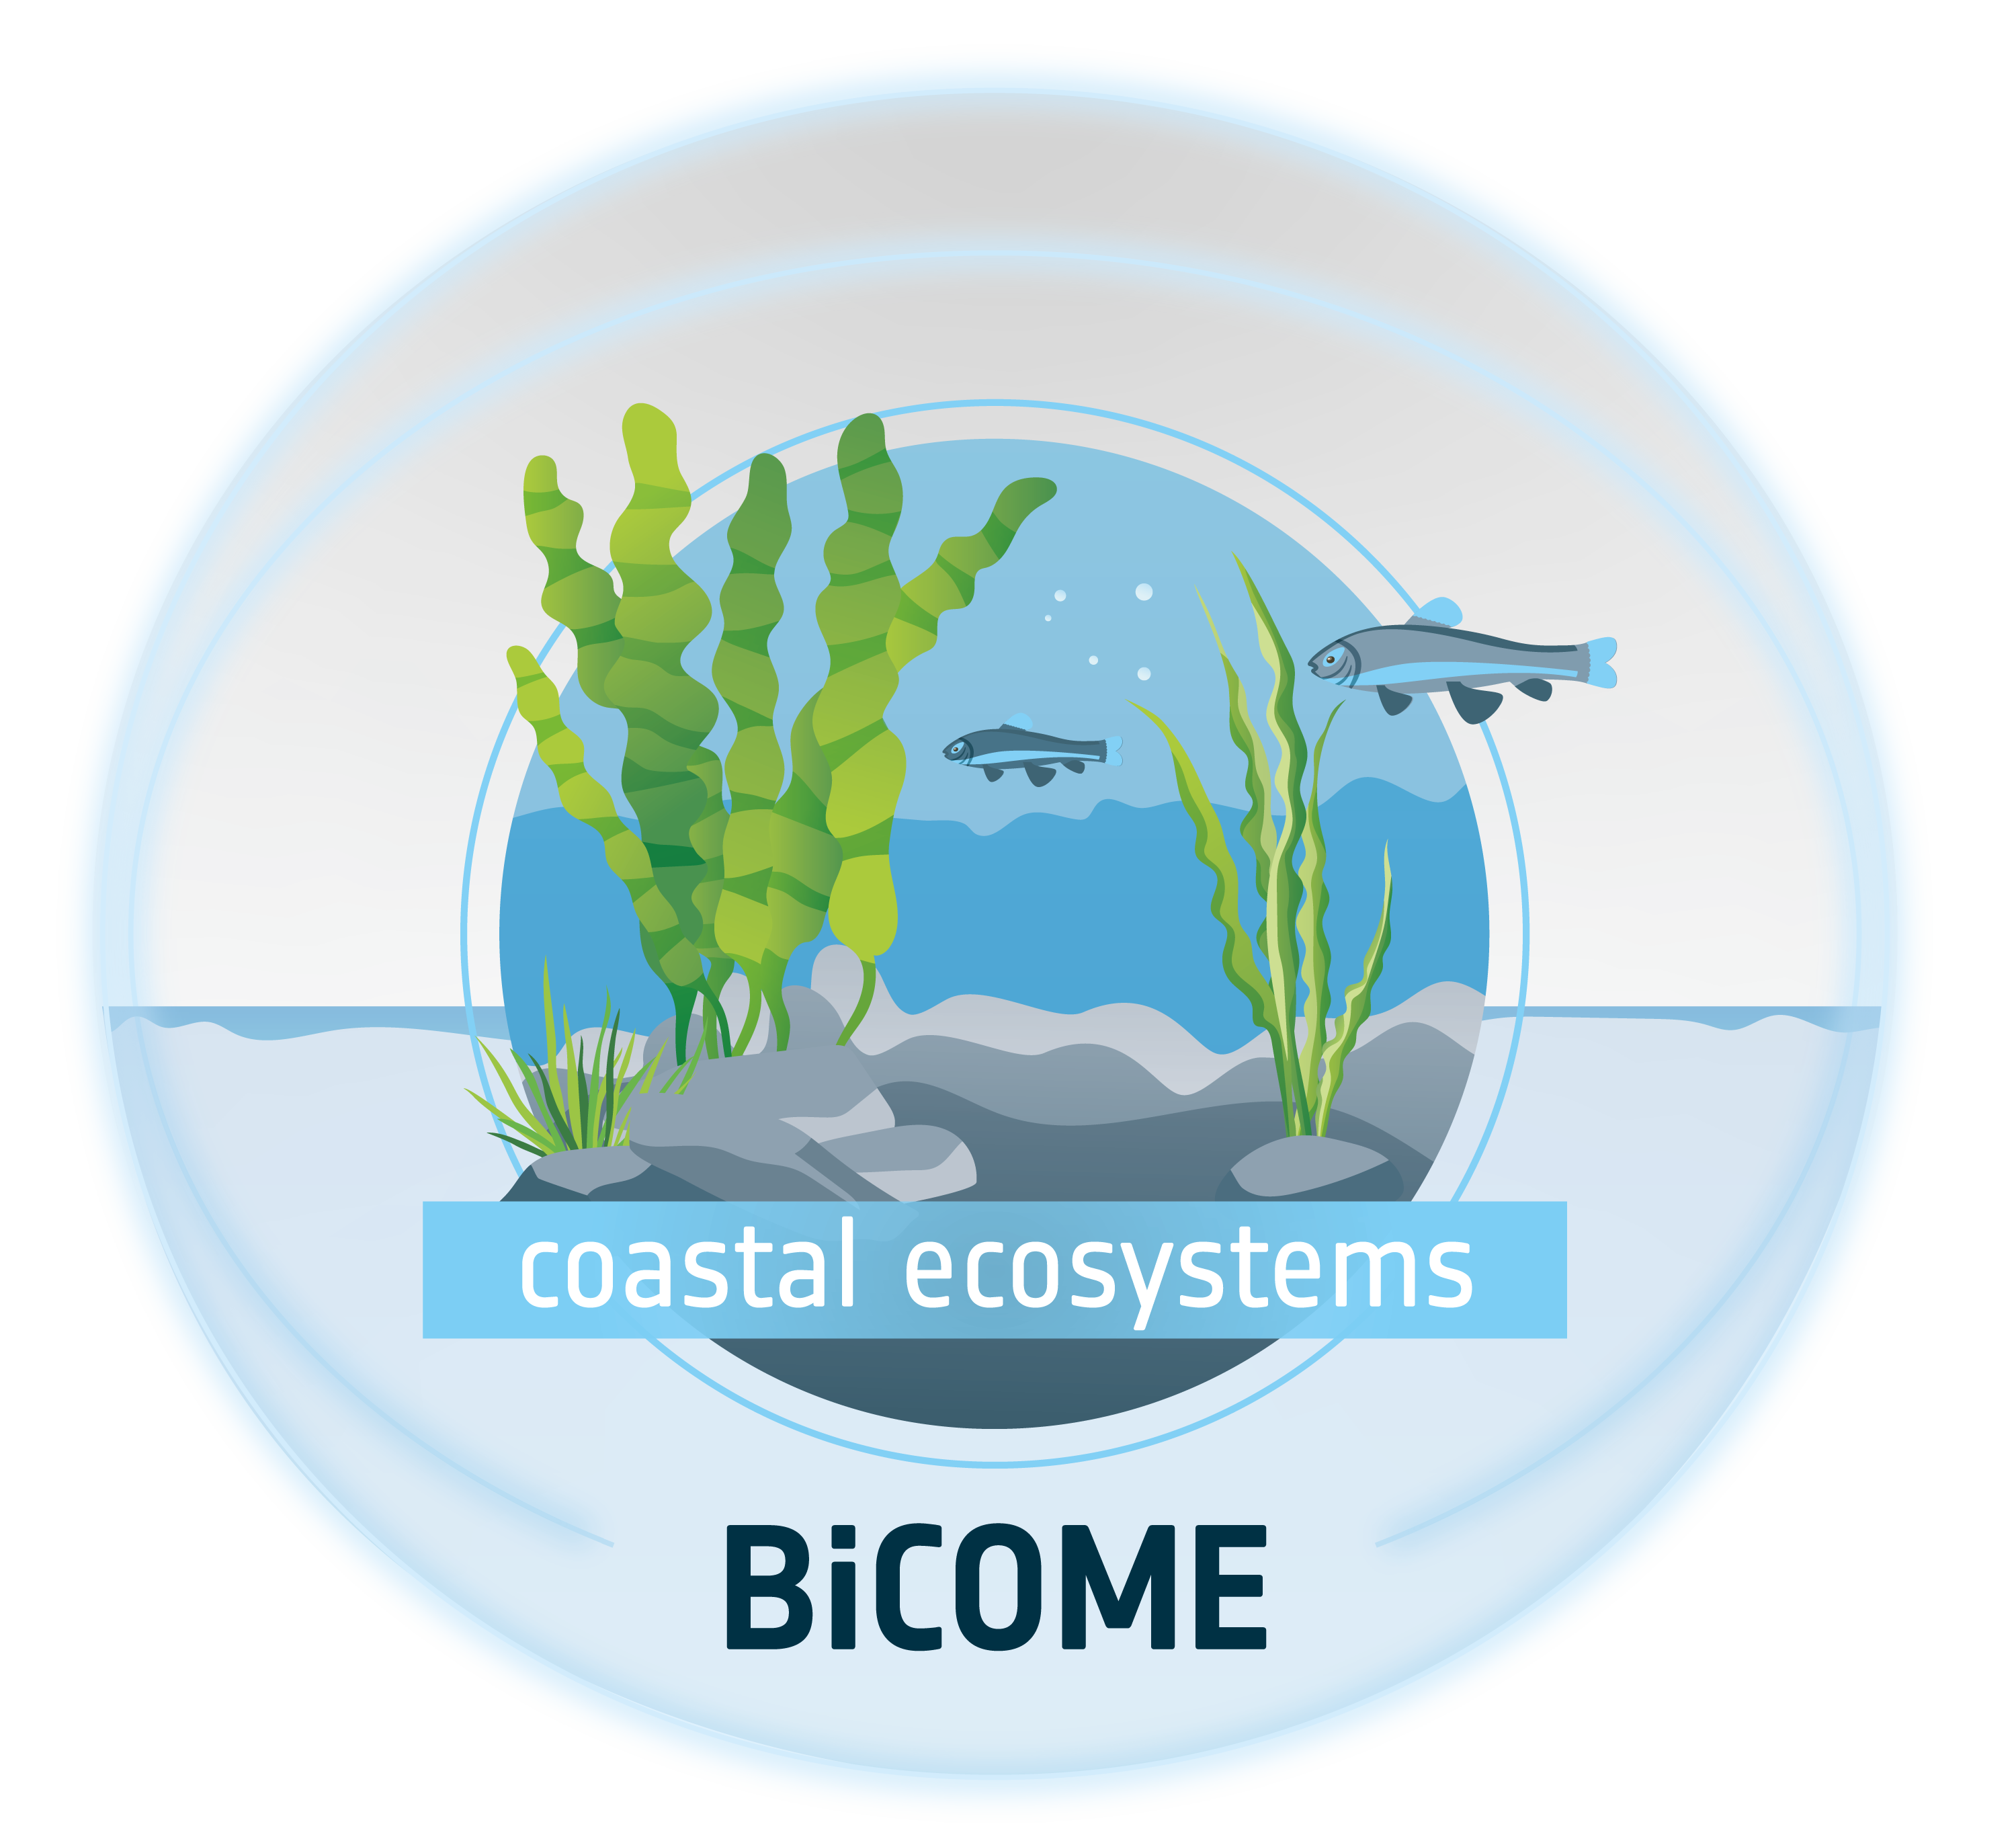
\includegraphics[width=0.4\linewidth,height=\textheight,keepaspectratio]{images/BiCOME Logo.png}
\end{center}
This thesis has been closely related to the european, ESA funded,
project \href{https://bicome.info}{BiCOME}. This project, led by the
Plymouth Marine Laboratory (\href{https://pml.ac.uk}{PML}) in
collaboration with the University of Nantes, the German Aerospace Center
(Deutsches Zentrum für Luft- und Raumfahrt,
\href{https://www.dlr.de/en}{DLR}) and
\href{https://hygeos.com/en/}{HYGEOS} has started in october 2021 and
has ended before the end of this thesis, in october 2023. It aimed to
demonstrate that Essential Biodiversity Variables (EBVs), relevant for
scientific and monitoring applications, can be obtained from
state-of-the-art remotely sensed reflectance close to the shoreline, and
that they can be scalable globally.

\begin{center}

\includegraphics[width=0.4\linewidth,height=\textheight,keepaspectratio]{images/ESA_Logo.png}
\end{center}

\begin{center}

\includegraphics[width=1\linewidth,height=\textheight,keepaspectratio]{images/logos_BICOME.png}
\end{center}

\newpage

\subsection*{Rewrite}\label{rewrite}
\addcontentsline{toc}{subsection}{Rewrite}

\begin{center}

\includegraphics[width=1\linewidth,height=\textheight,keepaspectratio]{images/Rewrite_banner.png}
\end{center}

Part of the thesis is related to the REWRITE project, led by Nantes
University and funded by the European Union. This project involves 24
partners across 14 countries and focuses on 10 demonstration sites. Its
aim is to promote the adaptation of the innovative conservation approach
known as `rewilding' as a nature-based solution for restoring Europe's
intertidal areas.

\begin{center}

\includegraphics[width=0.4\linewidth,height=\textheight,keepaspectratio]{images/EU_Logo.png}
\end{center}

\subsection*{InvaSea}\label{invasea}
\addcontentsline{toc}{subsection}{InvaSea}

Part of the thesis is related to the InvaSea project, founded by the
French National Centre for Space Studies (CNES). It aims to proves the
capacity of remote sensing to map the presence of the alien invasive
species \emph{Gracilaria vermiculophylla} in french and spanish
estuaries.

\begin{center}
\includegraphics[width=0.4\linewidth,height=\textheight,keepaspectratio]{images/cnes_logo.png}
\end{center}

\renewcommand{\chaptertopimage}{Chapter1/img/seagrasses.png}
\renewcommand{\chapterbottomimage}{Chapter1/img/fish_farm_psd.png}

\newpage\null\thispagestyle{empty}\newpage



%----------------------------------------------------------------------------------------
% ABSTRACT PAGE
%----------------------------------------------------------------------------------------
\startonleftwithgap
\newgeometry{top=0.5in, bottom=0.5in, left=0.5in, right=0.5in}
\pagestyle{plain}
\thispagestyle{empty}

\renewcommand{\familydefault}{\sfdefault} % Use sans-serif font throughout the document

\begin{tikzpicture}[remember picture, overlay]
    % Fill the triangle with the updated pattern
    \fill[pattern={Lines[angle=-45,distance={0.15cm}, line width=0.8pt]}, pattern color=greenTriangle]
        ([shift={(0,23.09cm)}]current page.south west) -- ++(0,4.19) -- ++(7.41,-2.095) -- cycle; % Triangle coordinates

\end{tikzpicture}

\begin{tabularx}{\textwidth}{X X} % Two equally spaced columns
  \centering
\includegraphics[height=2cm]{LogoED.png} & 
  \centering
\includegraphics[height=2cm]{LogoUN.jpg} \\
\end{tabularx} 

\vspace{1cm}

\noindent\textcolor[HTML]{2DA86A}{\rule{\textwidth}{5pt}}

\vspace{1cm}

\parbox{17cm}{

{{\fontsize{11}{15}\selectfont \textcolor{greenText}{\textbf{Titre :}}}}
{\fontsize{11}{15}\selectfont Caractérisation de la Végétation Intertidale sur les Côtes Européennes à l'Aide de la Télédétection Multi-Échelle en Réponse aux Pressions Naturelles et Anthropiques}} \\

{\fontsize{11}{15}\selectfont \textbf{Mots Clés:}}
{\fontsize{11}{15}\selectfont {Télédetection, Drones, Intertidale, Végétation, Multispectral}}

\parbox{17cm}{
\begin{multicols}{2}
{\fontsize{11}{15}\selectfont \textbf{Résumé:}}
{\fontsize{10}{14}\selectfont {La végétation intertidale joue un rôle clé dans les écosystèmes côtiers en stabilisant les sédiments, en abritant la biodiversité et en contribuant au cycle du carbone. Ce travail examine comment les approches de télédétection multi-échelles peuvent relever les défis de la surveillance et de la gestion de ces écosystèmes soumis à des pressions naturelles et anthropiques. En combinant des données issues de drones et de satellites, cette étude démontre l’efficacité de la télédétection multispectrale et hyperspectrale pour distinguer les zostères et les macroalgues dans les zones intertidales européennes. Les techniques d’apprentissage automatique sont mises en avant pour leur capacité à améliorer la précision des classifications et à relier les schémas de végétation aux gradients environnementaux, tels que l’altitude des marées et la stabilité des sédiments. Des expériences en laboratoire et des données de terrain soulignent l’impact des vagues de chaleur sur la santé de la végétation, fournissant des informations sur les réponses spectrales associées au stress et des indicateurs potentiels pour une détection précoce. Des analyses historiques révèlent également comment les activités humaines, telles que l’aquaculture, influencent la répartition de la végétation et la dynamique des écosystèmes au fil du temps. Cette approche intégrée souligne le potentiel de la télédétection pour capturer les schémas spatiaux et temporels de la biodiversité intertidale. Les résultats ont des implications majeures pour le suivi de la résilience des habitats, l’orientation des efforts de conservation et l’élaboration de politiques visant à atténuer les impacts du changement climatique et des activités humaines sur les environnements côtiers.}}
\end{multicols}
}

\noindent\textcolor[HTML]{2DA86A}{\rule{\textwidth}{5pt}}

\parbox{17cm}{

{{\fontsize{11}{15}\selectfont \textcolor{greenText}{\textbf{Title :}}}}
{\fontsize{11}{15}\selectfont Characterization of Intertidal Vegetation on European Coasts Using Multi-Scale Remote Sensing in Response to Natural and Anthropogenic Pressures}} \\

{\fontsize{11}{15}\selectfont \textbf{Keywords :}}
{\fontsize{11}{15}\selectfont {Remote Sensing, Drones, Intertidal, Vegetation, Multispectral}}

\parbox{17cm}{
\begin{multicols}{2}
{\fontsize{11}{15}\selectfont \textbf{Abstract :}}
{\fontsize{10}{14}\selectfont {Intertidal vegetation plays a key role in coastal ecosystems by stabilizing sediments, hosting biodiversity, and contributing to carbon cycling. This work examines how multi-scale remote sensing approaches can address challenges in monitoring and managing these ecosystems under natural and anthropogenic pressures. Combining drone and satellite data, this study demonstrates the effectiveness of multispectral and hyperspectral remote sensing in distinguishing seagrasses, macroalgae, across European intertidal zones. Machine learning techniques are highlighted for their ability to enhance classification accuracy and link vegetation patterns to environmental gradients, such as tidal elevation and sediment stability. Laboratory experiments and field data emphasize the impact of heatwaves on vegetation health, providing insights into the spectral responses associated with stress and potential metrics for early detection. Historical analyses further reveal how human activities, such as aquaculture, influence vegetation distribution and ecosystem dynamics over time. This integrated approach underscores the potential of remote sensing for capturing spatial and temporal patterns in intertidal biodiversity. The findings have broad implications for monitoring habitat resilience, guiding conservation efforts, and informing policies aimed at mitigating the impacts of climate change and human activities on coastal environments.}}
\end{multicols}
}

% \begin{tikzpicture}[remember picture, overlay]
%     % Fill the triangle with the updated pattern
%     \fill[pattern={Lines[angle=-45,distance={0.15cm}, line width=0.8pt]}, pattern color=greenTriangle]
%         ([shift={(21,1)}]current page.south west) -- ++(0,2.75) -- ++(-5.55,-1.375) -- cycle; % Triangle coordinates
% 
% \end{tikzpicture}
% 
% \begin{tikzpicture}[remember picture, overlay]
%     % Fill the triangle with the updated pattern
%     \fill[pattern=crosshatch dots, pattern color=greenTriangle]
%         ([shift={(0,1)}]current page.south east) -- ++(-5.55,0) -- ++(0,1.375) -- cycle; % Triangle coordinates
% \end{tikzpicture}

\restoregeometry
\end{document}
